% Two-column technical report (layout aligned with clinical_text_simplification/report).
% Build: cd report && pdflatex main && pdflatex main. Manual thebibliography; no BibTeX.
% Figures via \graphicspath{{../results/}}.
\documentclass[11pt,a4paper]{article}

\usepackage[a4paper,left=2.5cm,right=2.5cm,top=2.5cm,bottom=2.5cm,columnsep=0.6cm]{geometry}
\usepackage[british]{babel}
\usepackage[T1]{fontenc}
\usepackage[utf8]{inputenc}
\usepackage{times}
\usepackage[protrusion=true,expansion=false]{microtype}
\usepackage{booktabs}
\usepackage{amsmath,amssymb}
\usepackage{array}
\usepackage{tabularx}
\usepackage{graphicx}
\usepackage{xurl}
\usepackage{ragged2e}
\usepackage{dblfloatfix}
\usepackage{cuted}
\graphicspath{{../results/}}
\usepackage{caption}
\captionsetup{font=small,labelfont=bf,skip=2pt}
\setcounter{tocdepth}{2}
\usepackage[hidelinks,bookmarksnumbered=true,pdfusetitle]{hyperref}
\usepackage{bookmark}
\hypersetup{
  pdftitle={Register divergence in parallel CasiMedicos English: a corpus-linguistic audit (human vs Mistral)},
  pdfauthor={Darragh Kerins},
  linktoc=section,
}

\setlength{\emergencystretch}{2.8em}
\newcolumntype{Y}{>{\RaggedRight\arraybackslash}X}
\setlength{\hfuzz}{1.5pt}
\setlength{\parskip}{0pt}
\setlength{\parindent}{1em}

\newcommand{\code}[1]{\texttt{\small #1}}
\newcommand{\CA}{\emph{Corpus\,A}}
\newcommand{\CB}{\emph{Corpus\,B}}
\usepackage[htt]{hyphenat}

% Do not load titletoc here: it can break article ToC spacing (run-together ``1Introduction'').
\usepackage[toc]{appendix}
\usepackage{placeins}
\usepackage{needspace}
\usepackage{titlesec}
\titleformat{\section}{\normalfont\large\bfseries}{\thesection}{0.5em}{}
\titleformat{\subsection}{\normalfont\normalsize\bfseries}{\thesubsection}{0.5em}{}
\titleformat{\subsubsection}{\normalfont\normalsize\itshape}{\thesubsubsection}{0.5em}{}
\titleformat{\paragraph}[hang]{\normalfont\normalsize\bfseries}{}{0em}{\quad}
\titlespacing*{\section}{0pt}{8pt}{3pt}
\titlespacing*{\subsection}{0pt}{6pt}{2pt}
\titlespacing*{\subsubsection}{0pt}{5pt}{2pt}
\titlespacing*{\paragraph}{0pt}{4pt}{1.5pt}
\title{\textbf{Register divergence in parallel CasiMedicos English:\\
A corpus-linguistic audit of MCQ explanations \mbox{(human vs.\ Mistral)}}}
\author{Darragh Kerins \\ University of the Basque Country (UPV/EHU) \\ \url{drussell001@ikasle.ehu.eus}}
\date{}

\begin{document}
\begin{@twocolumnfalse}
\maketitle
\begin{abstract}\noindent
We analyse 117 paired MCQ justifications from CasiMedicos English \cite{casimedicos}: in each pair, the published human explanation and a Mistral rewrite both justify the same correct option. The human texts read as exam-focused justification; the model texts read more like explanatory clinical prose, with more hedging. Taken together, those patterns imply that treating lexical overlap with human keys as the default stand-in for ``clinical'' quality can mislead unless the register of the gold text is stated explicitly.
\end{abstract}
\vspace{0.5em}
\begingroup
\setcounter{tocdepth}{1}% sections only here, so the ToC fits on page~1 with the abstract
\small\tableofcontents\par
\endgroup
\setcounter{tocdepth}{2}% restore for any later ToC-dependent layout
\vspace{0.5em}
\end{@twocolumnfalse}
\twocolumn
\raggedbottom
\setcounter{dbltopnumber}{2}
\renewcommand{\dbltopfraction}{0.95}
\renewcommand{\textfraction}{0.08}
\renewcommand{\topfraction}{0.92}
\renewcommand{\floatpagefraction}{0.85}

\section{Introduction}

This paper shows that when both human explanations and Mistral outputs are written for the same correct multiple-choice answer, the differences between them are better explained by \textbf{register divergence} than by simple simplification of the human text.

By register divergence, we mean a consistent difference in how the texts are written: in their grammar, phrasing, and level of certainty. The human explanations tend to be written in an exam-focused style, aimed at justifying the correct option. The Mistral outputs instead tend to read more like explanatory clinical prose, with more general description and more hedging. Importantly, these differences do not reflect changes in the underlying diagnosis. This use of \emph{register} sits within corpus-linguistic work on situational variation \cite{biber1995,ferguson1983,kilgarriff2001}.

By \textbf{simplification}, in contrast, we would mean something narrower: shorter texts, less clinical detail, or a reduced lexical range relative to the human key. That expectation is already undermined by the token counts: \CB{} runs about 48\% \emph{longer} than \CA{} over the 117 strict pairs (Section~\ref{sec:res-length}, Table~\ref{tab:corpus-tokens}), which falsifies a compression-style reading of the model side rather than leaving it implicit.

Both human and model outputs are drawn from the same CasiMedicos English dataset \cite{casimedicos}, where each case is linked to a fixed correct answer. Because the answer is held constant, differences in wording are interpreted here as differences in communicative style, not differences in clinical correctness.

Section~\ref{sec:results} presents the analysis in detail: lexical and frequency patterns, patient framing, hedging, a validation check on the ontology linkage, and a boundary test under an unkeyed condition. Appendix~\ref{app:snomed-details} gives the full SNOMED-based analysis; Appendix~\ref{app:impl} gives reproducibility details; branch-pair aggregates are Appendix~\ref{app:branch}.

\section{Data and methods}
\label{sec:methods}

\subsection{Materials, keyed design, and measures}
\label{sec:case-layout}
We use the CasiMedicos-Arg English test split \cite{casimedicos} because each row supplies expert-written MCQ justifications tied to a single keyed correct answer: once that answer is held fixed, paired rewrites can be read as differing in register and packaging rather than in which diagnosis is defended. The English test split lists 125 cases; the corpus build filters eight rows that do not yield usable paired justification text, leaving \textbf{117} non-empty paired files under \path{corpus\_a}/\path{corpus\_b}. \CA{} is the published expert justification; \CB{} is output from Mistral, an open-weight instruction-tuned model, run locally via Ollama with British-English prompts and a length cap. The two sides are \emph{keyed}: both see which option is correct, so differences in wording are not confounded with picking a different diagnosis. A forty-case unkeyed rerun (Section~\ref{sec:boundary}) checks whether the register profile depends on that cue alone.

Each row runs from vignette through justification. The model prompt stops before the human justification text; saved files keep model replies only (\CB) and human tails only (\CA). For AntConc, we merge options, answer line, and justification on one line per case so keyword and concordance searches see the same surface the model saw (file routing and rebuild steps: Appendix~\ref{app:impl}).

We quantify length and Zipf profiles (NLTK stoplist), a fixed hedging lexicon (markers per 1\,000 tokens), TF--IDF on lemmas attested in both sides, and AntConc log-likelihood keywords, MI collocations ($\pm 5$ tokens), and KWIC. SNOMED~CT linkage via scispaCy \cite{snomed2026,neumann2019} is summarised in the Results where it matters for interpretation; full linkage tables and audits are Appendix~\ref{app:snomed-details}.

\FloatBarrier
\section{Results}
\label{sec:results}

\noindent Results follow this order: lexical and frequency patterns; patient framing; hedging; ontology validation with a short robustness summary; then a boundary check under an unkeyed condition (Section~\ref{sec:boundary}).

\subsection{Lexical and frequency distribution}\label{sec:res-lexfreq}\label{sec:antconc}

\noindent\textit{Length and tokens.}\label{sec:res-length}\quad
\CB{} runs about 48\% longer in tokens than \CA{} over 117 strict pairs; token totals are in Table~\ref{tab:corpus-tokens}.

\begin{table}[htbp]
\centering
\small
\caption{Token totals (117 cases).}
\label{tab:corpus-tokens}
\begin{tabular}{@{}lr@{}}
\toprule
 & Tokens \\
\midrule
\CA{} (human) & 10\,009 \\
\CB{} (model) & 14\,832 \\
\bottomrule
\end{tabular}
\end{table}

\Needspace{9\baselineskip}
\noindent\textit{Zipf and overall shape.}\quad
Figure~\ref{fig:zipf} plots Zipf ranks after stopword removal: \CA{} concentrates mass on exam-facing lemmas; \CB{} on expository clinical types. Together, greater length and shifted frequency mass support the introductory contrast: the model expands and redistributes material toward a clinical-expository profile rather than compressing the human key.

\begin{figure*}[tb]
\centering
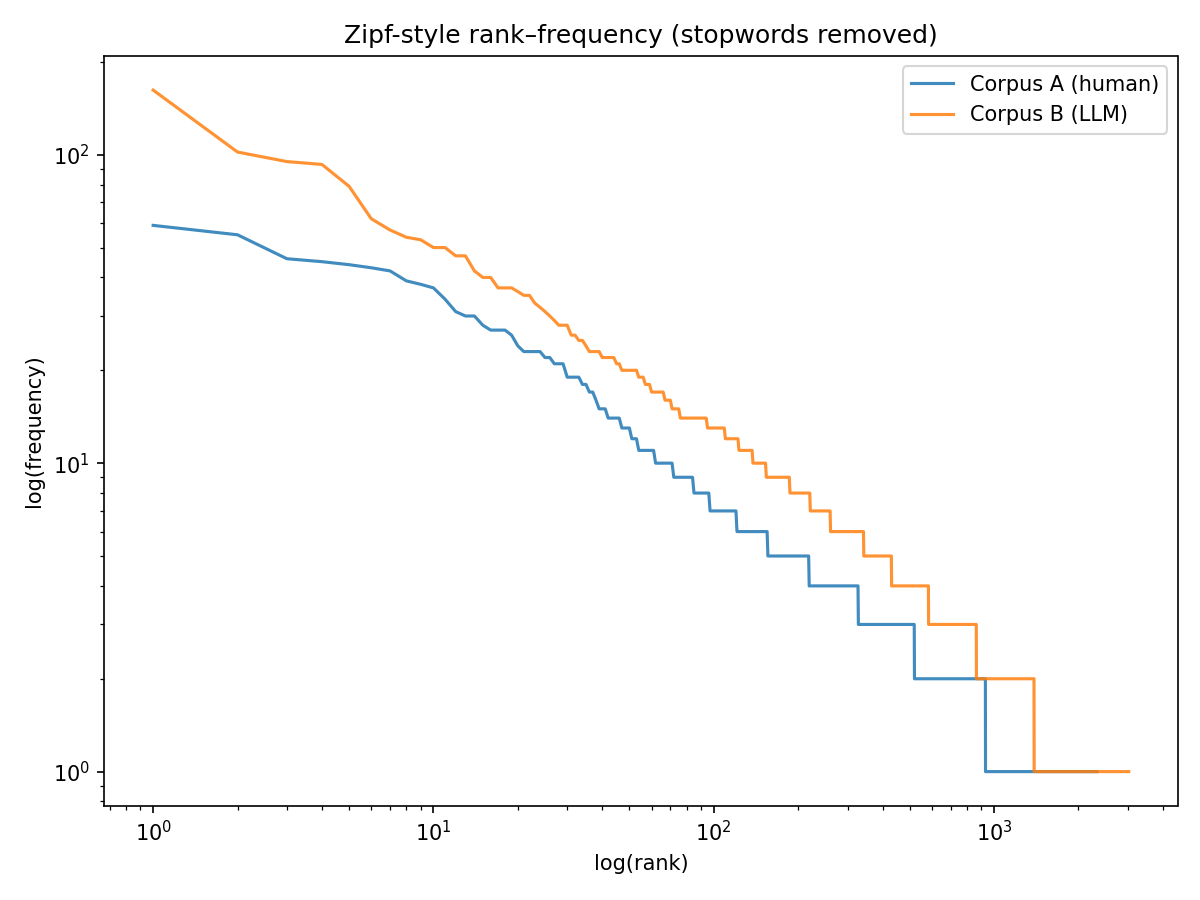
\includegraphics[width=0.96\textwidth]{corpus_frequency/zipf_rank_frequency_loglog.png}
\caption{Zipf (log--log): pooled rank vs frequency after stopword removal.}
\label{fig:zipf}
\end{figure*}

\noindent\textit{TF--IDF, keywords, and collocations.}\label{sec:res-register}\quad
TF--IDF on the 1385 lemmas attested in both corpora highlights profile differences without requiring full vocabulary overlap. Log-likelihood keywords, MI collocations, and KWIC are all computed on the same merged AntConc strict-pair lines, so they \emph{corroborate} the same surface profile rather than supplying three independent samples. Tables~\ref{tab:kw-b} and~\ref{tab:kw-a} list keyword groups ($\mathrm{LL}>10.83$, $\approx p<0.001$) on those files.

\begingroup
\setlength{\tabcolsep}{5pt}
\renewcommand{\arraystretch}{1.22}
\begin{table}[htbp]
\centering
\small
\caption{Keyword groups overused in \CB{} vs.\ \CA{} as reference.}
\label{tab:kw-b}
\begin{tabularx}{\columnwidth}{@{}lY@{}}
\toprule
Theme & Examples (LL) \\
\midrule
Epistemic lexis & \emph{likely} (52.3), \emph{typically} (38.6), \emph{suggests} (32.9), \emph{consistent} (16.4), \emph{potential} (15.6) \\
Clinical nouns & \emph{presentation} (29.0), \emph{findings} (30.0), \emph{patient} (24.7), \emph{vignette} (12.4) \\
Scaffolding & \emph{While} (52.9), \emph{Although} (19.3), \emph{Given} (19.8) \\
MCQ form & \emph{Option} (60.4) \\
Evidential & \emph{support} (11.0), \emph{supports} (23.0) \\
\bottomrule
\end{tabularx}
\end{table}

\begin{table}[htbp]
\centering
\small
\caption{Keyword groups overused in \CA{} vs.\ \CB{} as reference.}
\label{tab:kw-a}
\begin{tabularx}{\columnwidth}{@{}lY@{}}
\toprule
Theme & Examples (LL) \\
\midrule
First-person & \emph{we} (130.2), \emph{We} (39.9), \emph{us} (47.1), \emph{have} (28.7) \\
MCQ meta & \emph{answer} (81.6), \emph{question} (48.3), \emph{correct} (40.0), \emph{one} (46.5), \emph{false} (15.4), \emph{discarded} (14.5) \\
Connectives & \emph{that} (53.8), \emph{so} (48.3), \emph{because} (37.9), \emph{since} (24.9) \\
Perception & \emph{think} (14.5), \emph{probably} (12.7), \emph{appear} (12.7), \emph{seems} \\
Modality & \emph{will} (27.5), \emph{must} (12.7) \\
Intensifiers & \emph{very} (45.3), \emph{only} (36.2), \emph{clear} (14.1) \\
\bottomrule
\end{tabularx}
\end{table}
\endgroup

\noindent Figure~\ref{fig:tfidf-gaps} gives the ten largest mean TF--IDF gaps in each direction; \CA{} loads exam-facing items (\emph{we}, \emph{answer}, \emph{it}), \CB{} coordinators and clinical nouns (\emph{and}, \emph{the}, \emph{diagnosis}).

\begin{figure*}[t]
\centering
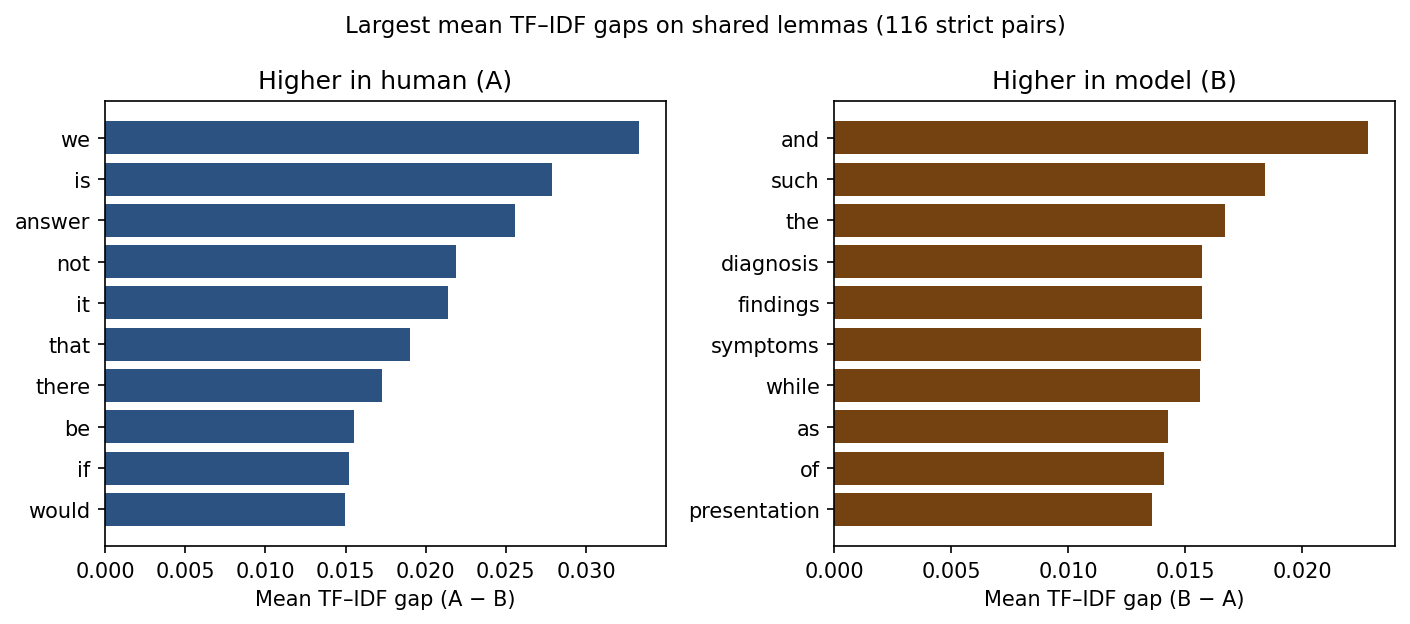
\includegraphics[width=0.96\textwidth]{report_figures/tfidf_gap_bars.png}
\caption{Largest mean TF--IDF gaps on shared lemmas (positive values indicate higher weight in Corpus~A).}
\label{fig:tfidf-gaps}
\end{figure*}

\noindent\textbf{Collocations} (MI window $\pm 5$, min.\ freq.\ 3) for focal lemmas:
\begin{itemize}\setlength\itemsep{1pt}
\item \textbf{\emph{answer}} --- A: stable ``The correct answer is $N$'' frame; B: no matching template at the same threshold.
\item \textbf{\emph{diagnosis}} --- sparse structure in A; B with \emph{most likely}, \emph{confirm}, \emph{support}.
\item \textbf{\emph{patient}} --- no A-side collocate above threshold; B: strong MI for possessive \emph{'s} with clinical-record nouns.
\item \textbf{\emph{treatment}} --- A: \emph{choice}, \emph{surgical}; B: \emph{first-line}, \emph{line}, \emph{antibiotic}.
\end{itemize}
\noindent One compact epistemic measure already separates the profiles: on the merged AntConc strict-pair exports (\path{antconc\_input/corpus\_a\_merged.txt}, \path{antconc\_input/corpus\_b\_merged.txt}), whitespace-delimited word counts (\texttt{wc -w}) give \emph{most likely} at $\approx$2.51 versus $\approx$0.60 per 1k words in \CB{} and \CA{} respectively---a ratio of about \textbf{4.2{:}1}. (Hedging in Section~\ref{sec:res-hedge} instead uses the pipeline's lowercase word-token regex on the per-case files; the two layers therefore share the same texts but not identical token totals.) KWIC in Section~\ref{sec:res-patient} shows how that item behaves in running text.

\noindent Lexis and phraseology therefore line up with two different interactional templates: option- and answer-oriented metalanguage on the human side versus clinical-record scaffolding on the model side. That contrast matches the exam-focused versus explanatory-clinical split set out in the Introduction, rather than a uniform shortening of the human key.

\FloatBarrier

\subsection{Patient framing and KWIC}\label{sec:res-patient}

\begingroup
\setlength{\tabcolsep}{5pt}
\renewcommand{\arraystretch}{1.12}
\begin{table*}[t]
\centering
\small
\caption{\emph{patient}: frequency and structure (merged strict-pair files).}
\label{tab:patient}
\begin{tabularx}{\textwidth}{@{}l>{\RaggedRight\arraybackslash}p{0.33\textwidth}>{\RaggedRight\arraybackslash}Y@{}}
\toprule
Feature & \CA{} (human) & \CB{} (model) \\
\midrule
Raw frequency & 48 hits & 153 hits \\
Per 1k tokens & 4.77 & 10.38 \\
Dominant structure & Indefinite narrative: \emph{a patient with X} & Possessive expository: \emph{the patient's X} \\
Dominant openers & \emph{We are described / presented / faced with a patient with\ldots} & \emph{Given the patient's\ldots}; \emph{Based on the patient's\ldots};\newline sentence-initial \emph{The patient's\ldots} \\
Function & Exam-oriented justification & Expository clinical framing toward diagnosis or management \\
\bottomrule
\end{tabularx}
\end{table*}
\endgroup

\FloatBarrier
\begin{strip}
\noindent
\begin{minipage}[t]{0.475\textwidth}\RaggedRight
Table~\ref{tab:patient} summarises frequency and syntactic framing for \emph{patient}. \CB{} favours opener $+$ \emph{the patient's} $+$ conclusion; \CA{} favours \emph{a patient with X} scene-setting (raw hits ratio $\approx 2.2{:}1$, higher in \CB{}).
\end{minipage}\hfill
\begin{minipage}[t]{0.475\textwidth}\RaggedRight
\noindent\textbf{Concordance (KWIC).}\par
\small
\noindent\CA{} (human):
\begin{quote}\RaggedRight
``We have before us a patient with neuropathic pain, which due to the origin of the tumor, is most likely due to involvement of the celiac plexus.''

``We are faced with polyuria. Initially we rule out diabetes mellitus (our patient has a normal blood glucose of 96mg/dl).''
\end{quote}
\medskip
\noindent\CB{} (model):\par\nobreak
\begin{quote}\RaggedRight
``Given the patient's age, comorbidities, and the clinical findings of joint swelling, varus deformity, limited [\ldots]''

``The patient's presentation aligns with Systemic Lupus Erythematosus (SLE), a condition that typically requires [\ldots]''
\end{quote}
\end{minipage}
\end{strip}

\vspace{2.8mm}
\noindent\textbf{Epistemic \emph{most likely}.} The corpus-level rate ($\approx$\textbf{4.2{:}1}, Section~\ref{sec:res-register}) shows up locally in these excerpts. \CA{} still carries occasional Spanish-examination lemmas (\emph{MIR}, \emph{SEGO}) absent from \CB{}.

Patient reference and concordance lines show how the same clinical referent is staged for different addressees: scene-setting and exam voice versus possessive, evidence-led clinical prose. That staging difference changes who the text is ``for'' while the keyed diagnosis stays fixed, which is what a register-based contrast predicts.

\FloatBarrier

\subsection{Hedging density}\label{sec:res-hedge}
Lexicon-based epistemic markers rise from 20.78 to 36.81 per 1k tokens pooled (Table~\ref{tab:hedge-pooled}). Counts use the saved per-case \CA{} and \CB{} justification files rather than the merged AntConc line, but they still describe the same 117 pairs, so they corroborate---without independently replicating---the AntConc-based layers in Section~\ref{sec:res-register}.

\begin{table}[htbp]
\centering
\small
\caption{Pooled hedging (markers per 1k tokens).}
\label{tab:hedge-pooled}
\begin{tabular}{@{}lr@{}}
\toprule
 & /1k tokens \\
\midrule
\CA{} (human) & 20.78 \\
\CB{} (model) & 36.81 \\
\bottomrule
\end{tabular}
\end{table}

\noindent Figure~\ref{fig:hedge-bar} summarises overall density by corpus.

\begin{figure}[htbp]
\centering
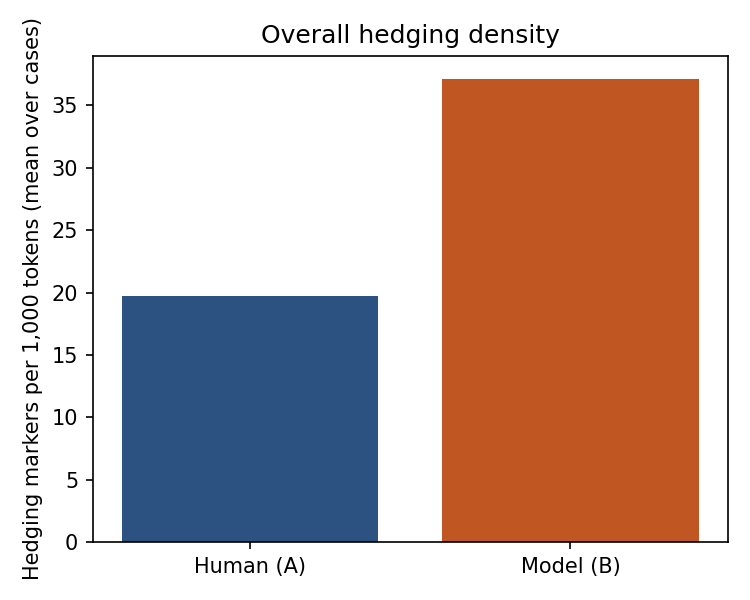
\includegraphics[width=\columnwidth]{hedging/specialty_lexicon_tagging/bar_overall_human_vs_model.png}
\caption{Hedge density (markers per 1k tokens), all 117 cases.}
\label{fig:hedge-bar}
\end{figure}

\noindent Table~\ref{tab:hedging} gives a coarse-area excerpt (small-$n$ rows are indicative only).

\begin{table}[htbp]
\centering
\small
\caption{Hedging by coarse area ($\Delta =$ model $-$ human).}
\label{tab:hedging}
\begin{tabular}{@{}lrrrr@{}}
\toprule
Area & $n$ & Human & Model & $\Delta$ \\
\midrule
All cases (pooled) & 117 & 20.8 & 36.8 & 16.0 \\
General medicine & 47 & 22.2 & 35.7 & 13.6 \\
Obstetrics \& gyn. & 7 & 0.0 & 39.2 & 39.2 \\
Nephrology \& urol. & 7 & 19.9 & 30.2 & 10.3 \\
Respiratory & 7 & 28.8 & 51.4 & 22.6 \\
Cardiovascular & 6 & 14.0 & 43.8 & 29.8 \\
\bottomrule
\end{tabular}
\end{table}

\noindent The obstetrics and gynaecology row (human 0.0 vs.\ model 39.2 per 1k tokens, $n=7$) rests on a tiny subsample and should not be read as a stable specialty effect. With $n=7$, a human rate of zero may reflect sparse lexicon matches as much as a genuinely categorical tone; either reading remains anecdotal at this cell size.

Higher pooled hedging on \CB{} is part of the same register shift: the model routinely softens and generalises claims where the human key often commits to a single exam-facing line of reasoning. In other words, epistemic stance moves with the packaging, which supports the divergence reading rather than a story in which the model simply strips certainty from the human wording.

\FloatBarrier

\subsection{Ontology validation and robustness checks}\label{sec:snomed}
A \emph{shallow linker artefact} would arise if the pipeline treated surface strings naively---for example, if the same span always received the same SNOMED depth regardless of corpus, or if depth summaries tracked identical spellings only. In the worst case, an asymmetric linker could produce fake ``depth'' contrasts that mimic register differences in Sections~\ref{sec:res-lexfreq}--\ref{sec:res-patient} without any change in how clinicians actually write. We therefore use RF2 linkage checks \cite{snomed2026,neumann2019} to ask whether the lexical and framing gaps in Sections~\ref{sec:res-lexfreq}--\ref{sec:res-hedge} could plausibly be reduced to that sort of mechanical side effect.

These checks do not adjudicate clinical correctness; they bound linkage artefacts so the register contrast is not dismissed as a trivial NER quirk. Table~\ref{tab:verdict} summarises hypotheses, instruments, and short verdicts; branch-pair aggregates and full diagnostics remain Appendix~\ref{app:snomed-details} and Appendix~\ref{app:branch}.

\begingroup
\setlength{\tabcolsep}{4.5pt}
\renewcommand{\arraystretch}{1.12}
\begin{table*}[t]
\centering
\small
\caption{Hypotheses and short verdicts (117 strict pairs; unkeyed ablation $n=40$).}
\label{tab:verdict}
\begin{tabularx}{\textwidth}{@{}>{\RaggedRight\arraybackslash}p{3.55cm}>{\RaggedRight\arraybackslash}p{4.65cm}Y@{}}
\toprule
Hypothesis & Instrument & Verdict \\
\midrule
Same-string depth asymmetry & SNOMED depths, $n=411$ shared strings & Not applicable (same-string table). \\
Referential consistency & Branch grid $>872$k; two 48-row review CSVs & Details in Appendix~\ref{app:snomed-details}; grid Appendix~\ref{app:branch}. \\
Lexical gap & Zipf, TF--IDF, token totals & Supported (length; lexical profile). \\
Keyed-only artefact & 40-case unkeyed \CB{} (Table~\ref{tab:ablation}) & Not supported on subsample. \\
Lexical + hedging profile & Keywords, MI, KWIC, hedging & Supported (Sections~\ref{sec:res-lexfreq}--\ref{sec:res-hedge}). \\
\bottomrule
\end{tabularx}
\end{table*}
\endgroup

\subsection{Boundary check (unkeyed condition)}\label{sec:boundary}
Forty stratified cases were rerun with the correct option withheld from the Mistral prompt while \CA{} stayed fixed. If the register profile were a pure artefact of seeing the keyed option, pooled hedging and epistemic \emph{most likely} should move sharply toward the human side when that cue is removed. They do not (Table~\ref{tab:ablation}), which supports treating the register shift as stable under this perturbation rather than as a keyed-only quirk. Independently of that stability, Table~\ref{tab:ablation} shows how wide the keyed hedging gap already is: \CA{} sits near 21 markers per 1\,000 tokens on this slice, while keyed \CB{} sits near 38, so the model side is not merely edging above the human baseline. The subsample is small; the row is a falsification-oriented bound, not a replication.

\begingroup
\setlength{\tabcolsep}{6pt}
\renewcommand{\arraystretch}{1.1}
\begin{table*}[t]
\centering
\small
\caption{Boundary check: 40-case unkeyed \CB{} (\CA{} unchanged; $\Delta =$ unkeyed $-$ keyed on \CB{}).}
\label{tab:ablation}
\begin{tabular}{@{}lrrrr@{}}
\toprule
Measure & A & B key. & B unk. & $\Delta$ \\
\midrule
Hedge /1k tokens & 20.66 & 37.57 & 38.47 & $+0.90$ \\
\emph{most likely} /1k & 0.54 & 2.56 & 2.96 & $+0.40$ \\
SNOMED depth (mean) & 8.84 & 8.84 & 8.84 & 0.00 \\
\bottomrule
\end{tabular}
\end{table*}
\endgroup

\section{Discussion}
\label{sec:discussion}

\subsection{Register vs.\ accuracy}

The findings support the introduction: with the correct answer fixed, the two sides differ chiefly in \emph{how} that answer is argued for---stance, metalanguage, and patient framing---rather than in a straight shortening of the human text. Ontology checks in Table~\ref{tab:verdict} do not re-score clinical truth; they show the lexical contrast is not plausibly explained away as one shallow linker artefact.

\subsection{Limits of overlap-based evaluation}

Automatic evaluation of clinical NLP outputs often relies on lexical overlap metrics such as BLEU, ROUGE, and BERTScore, which score model text by its surface similarity to a human reference. In a medical MCQ setting, that usually means measuring how closely model justifications resemble expert-written keys. These scores are computationally convenient and widely used, but they carry a tacit assumption: that the reference instantiates the register one wants to reward. When it does not---or when that register is never stated---the metric can penalise valid outputs for being written differently, not for being wrong.

\textbf{Lexical or $n$-gram overlap with human examination keys is a weak proxy for clinical adequacy} in this setting. \CB{} reads like textbook-style exposition; \CA{} reads like examiner-facing justification. Scores that reward similarity to the key can therefore punish the wrong kind of difference: \CB{} is often lexically nearer to generic expository clinical prose than \CA{} is, yet further from the exam-facing stance of the key.

The roughly \textbf{4.2{:}1} imbalance for \emph{most likely} (Section~\ref{sec:res-register}) is one clear scalar example: it marks epistemic packaging, not a change of diagnosis under the keyed design.

Evaluations should say which register the gold standard encodes. Overlap-based metrics need phraseological companions. Where the key is treated as default ``clinical'' gold, that choice should be stated openly; otherwise valid clinical prose in another register may be marked down, and ``clinical'' quality may be reduced to a single number with no named audience.

\subsection{Implications for LLM evaluation}

Register varies along several dimensions at once \cite{biber1995,ferguson1983}. When the diagnosis is fixed, parallel texts let researchers separate agreement on the case from how the case is written. Keywords, collocations, and concordance lines bring out recurrent frames that a single overlap score can hide. Teams that tune only towards human keys risk missing a steady mismatch in packaging, even when surface word overlap looks acceptable.

Evaluators should name the register of the gold standard in the paper or rubric (exam key, textbook prose, chart note, etc.). They should report phraseological diagnostics---keywords, collocations, concordance---alongside $n$-gram or embedding overlap so packaging shifts are visible. Where possible, parallel corpora with a keyed correct option offer a clean way to hold clinical content constant while comparing form. Reviewers can then ask whether a ``clinical'' score is measuring stance and audience fit, not only proximity to a single gold string.
\FloatBarrier

\section{Scope and limitations}

Claims are limited to the English test split and to 117 strict pairs. As noted in Section~\ref{sec:res-register}, AntConc-derived layers corroborate one surface rather than triangulating independently. Ontology validation is string-level and audit-scoped (Appendix~\ref{app:snomed-details}). CasiMedicos is CC-BY; SNOMED CT RF2 is not redistributed here \cite{snomed2026}.

\section{Conclusion}

With the correct option fixed, Mistral output reads more like explanatory clinical prose---with stronger hedging and different patient framing---than the human key. The unkeyed check in Section~\ref{sec:boundary} suggests that profile is not only a side-effect of revealing the keyed option. The overall pattern implies that heavy reliance on lexical overlap with examination keys can misrank clinical-sounding model prose. Register should be treated as an explicit variable in LLM evaluation, not as a silent property of whatever text happens to serve as gold.

\noindent Gold standards should name their audience. Overlap metrics need phraseological companions. Packaging can diverge while the case stays fixed, and evaluators should expect that pattern when keys are written for an exam-facing reader.

\FloatBarrier
\phantomsection
\addcontentsline{toc}{section}{\protect\numberline{}References}
\begin{thebibliography}{99}
\footnotesize
\setlength\itemsep{1pt}
\setlength\parskip{0pt}
\bibitem{biber1995} Douglas Biber. 1995. \emph{Dimensions of Register Variation}. Cambridge University Press.
\bibitem{casimedicos} Ekaterina Sviridova, Anar Yeginbergen, Ainara Estarrona, Elena Cabrio, Serena Villata, and Rodrigo Agerri. 2024. CasiMedicos-Arg: A medical question answering dataset annotated with explanatory argumentative structures. In \emph{Proceedings of the 2024 Conference on Empirical Methods in Natural Language Processing (EMNLP)}, 18463--18475. \url{https://aclanthology.org/2024.emnlp-main.1026}. English split via HiTZ Hugging Face: \url{https://huggingface.co/datasets/HiTZ/casimedicos-arg}.
\bibitem{ferguson1983} Charles A. Ferguson. 1983. Medical discourse. \emph{Text}, 3(3):223--248.
\bibitem{kilgarriff2001} Adam Kilgarriff. 2001. Comparing corpora. \emph{Int.\ J.\ Corpus Linguistics}, 6(1):97--133.
\bibitem{neumann2019} Mark Neumann et al. 2019. scispaCy: Fast and robust biomedical NLP.
\bibitem{snomed2026} SNOMED International. SNOMED~CT Release Format~2 (RF2), international edition (continuously updated release). Accessed 16th April 2026. \url{https://www.snomed.org/}.
\end{thebibliography}

\clearpage
\begin{appendices}

\section{SNOMED linkage and audits}
\label{app:snomed-details}

This appendix documents SNOMED CT RF2 linkage outputs: entity tables, depth deltas on shared strings, optional CSV audits, and capped reviewer-model rows. \code{is\_a} depth presupposes mention alignment. Branch-pair counts are Appendix~\ref{app:branch}. The hypothesis--instrument summary is Table~\ref{tab:verdict} in Section~\ref{sec:snomed}; the unkeyed depth row matches Section~\ref{sec:boundary} (mean depth on entities resolvable in keyed \CA{}, keyed \CB{}, and unkeyed \CB{}, $n=106$).

\subsection{Pooled NER and same-string depth deltas}
\label{sec:app-verdict}
NER yields 1684 / 2572 distinct entity strings on A / B (concept match $\sim$74\%/72\%; depth-resolvable 58\%/56\%; mean depth 9.67 vs.\ 9.84). The 411 strings shared across corpora inherit one depth per side from the string-level table, so that slice cannot yield a within-string depth asymmetry. Figure~\ref{fig:snomed-hist} plots same-string depth deltas (\code{pair\_depths}).

\begin{figure*}[t]
\centering
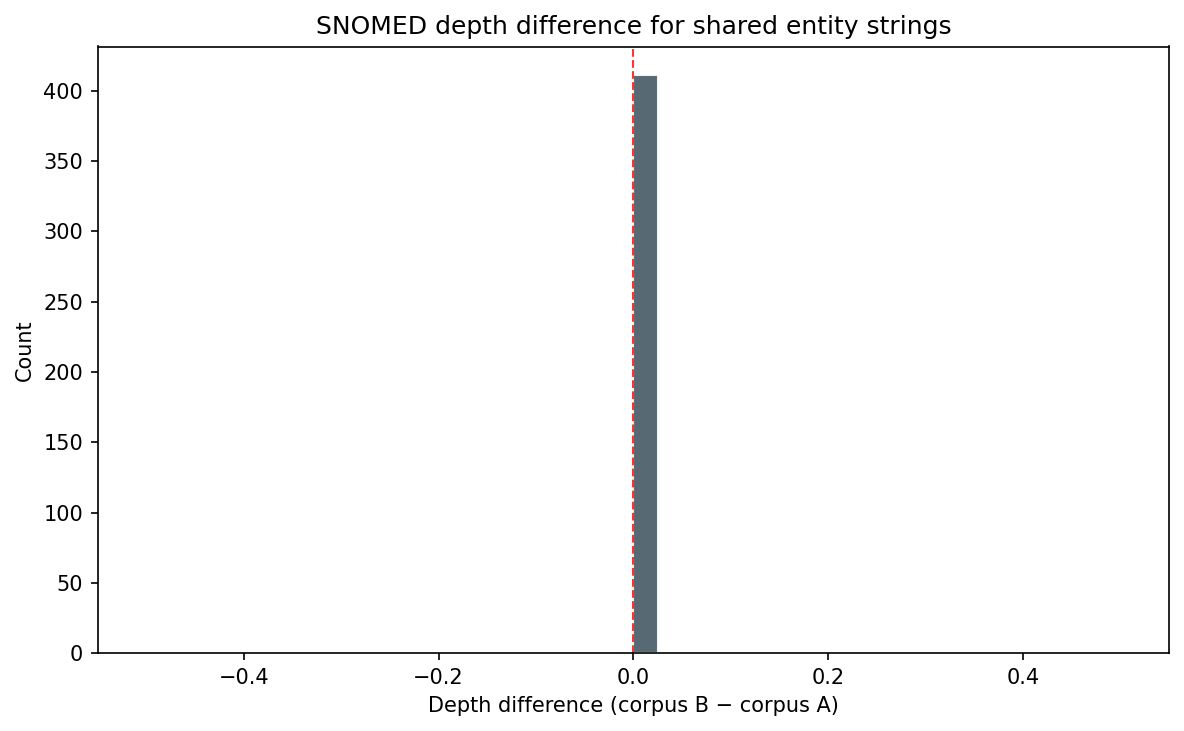
\includegraphics[width=0.72\textwidth]{snomed/hist_depth_difference_b_minus_a.png}
\caption{Same-string SNOMED depths: distribution of (depth B $-$ depth A) on paired shared entities (\code{pair\_depths}). Most mass at zero when linker agrees.}
\label{fig:snomed-hist}
\end{figure*}

\subsection{Vagueness-oriented ladder export}\label{sec:vague-op}
Per-case NER on both sides yields pairs of \emph{different} strings in strict RF2 \code{is\_a} relation with $\lvert \mathrm{depth\_a} - \mathrm{depth\_b} \rvert \geq 3$ (up to 20 pairs per file by depth gap). This is a taxonomic ladder, not coreference. Paths and optional LLM review seeds are listed in Appendix~\ref{app:impl}.

\subsection{Same-string Mistral audit (48 rows)}
Fixed-seed sample of overlapping entity strings; each row supplies the string plus short A/B context to the reviewer model. Counts: 44 \textsc{keep}, 2 \textsc{substitute}, 2 \textsc{incomparable}. Rubric: linker agreement on identical spellings.

\begin{table}[t]
\centering
\small
\caption{Mistral decisions on 48 sampled per-case same-string overlaps.}
\label{tab:llm}
\begin{tabular}{@{}lr@{}}
\toprule
Decision & Count \\
\midrule
\textsc{keep} & 44 \\
\textsc{substitute} & 2 \\
\textsc{incomparable} & 2 \\
\bottomrule
\end{tabular}
\end{table}

\subsection{Hierarchical is-a Mistral audit (48 rows)}
% Auto-generated by report/gen_report_figures.py — do not edit.
% Rebuild: python3 report/gen_report_figures.py
\def\LLMHierN{48}
\def\LLMHierKeep{1}
\def\LLMHierSub{45}
\def\LLMHierInc{2}


Second draw of $n=\LLMHierN{}$ rows from hierarchical seeds (subsection~\ref{sec:vague-op}): different strings, strict \code{is\_a} nesting, depth-gap filter, hierarchical rubric. Last exported counts: \LLMHierKeep{} \textsc{keep}, \LLMHierSub{} \textsc{substitute}, \LLMHierInc{} \textsc{incomparable}. Expected to differ from Table~\ref{tab:llm} (taxonomic edge $\neq$ pragmatic co-reference). Regeneration: Appendix~\ref{app:impl}.

\noindent A high \textsc{substitute} count on different strings means the reviewer model often rejects the taxonomic edge as the right pragmatic link for that mention in context; it does not invalidate same-string RF2 rows, but it cautions against treating hierarchical pairs as clinically aligned mentions without manual spot checks.

\begin{table}[t]
\centering
\small
\caption{Mistral decisions on $n=\LLMHierN{}$ sampled per-case hierarchical is-a seeds (different strings).}
\label{tab:llm-hier}
\begin{tabular}{@{}lr@{}}
\toprule
Decision & Count \\
\midrule
\textsc{keep} & \LLMHierKeep \\
\textsc{substitute} & \LLMHierSub \\
\textsc{incomparable} & \LLMHierInc \\
\bottomrule
\end{tabular}
\end{table}

\begin{figure*}[t]
\centering
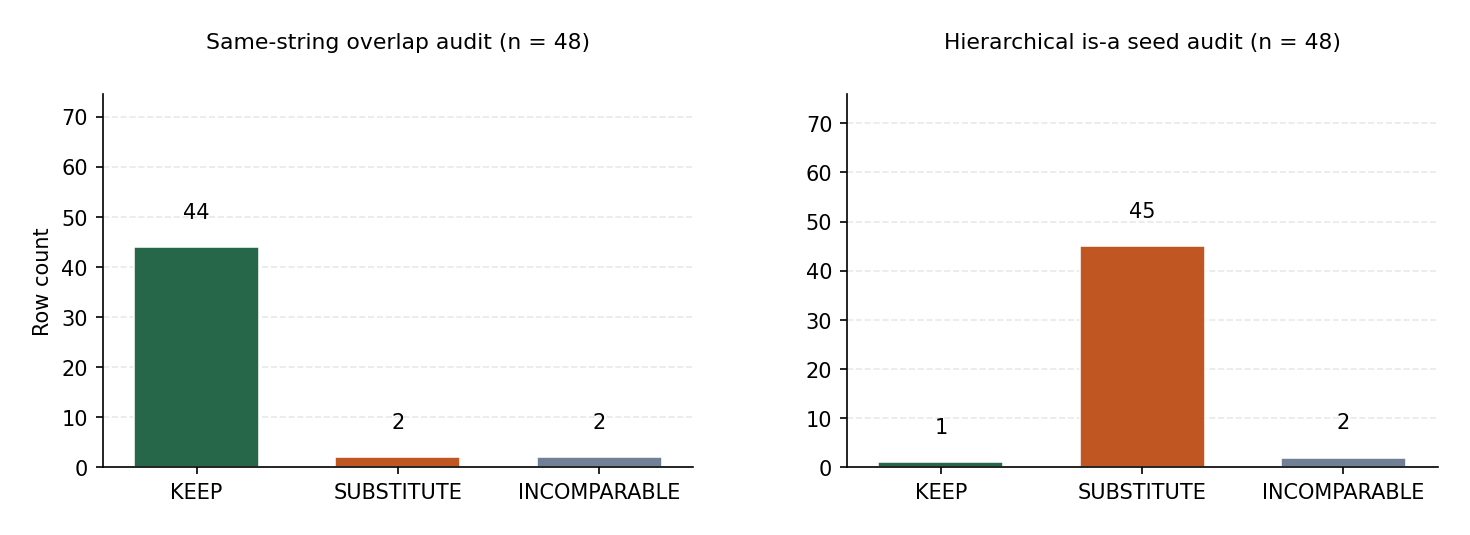
\includegraphics[width=0.92\textwidth]{report_figures/llm_audit_pair_bars.png}
\caption{Same-string overlap audit (Table~\ref{tab:llm}, left) and hierarchical is-a seed audit (Table~\ref{tab:llm-hier}, right).}
\label{fig:llm-pair}
\end{figure*}

\section{Implementation notes and reproducibility}
\label{app:impl}

\subsection{Pipeline mapping}
Table~\ref{tab:prep-map} routes raw row parts (vignette through expert justification) to the keyed prompt and to Corpus~A/Corpus~B files.

\begin{table}[t]
\centering
\footnotesize
\caption{Pipeline mapping from each CasiMedicos row to prompts and saved files.}
\label{tab:prep-map}
\begin{tabularx}{\columnwidth}{@{}p{0.28\columnwidth}Y@{}}
\toprule
Piece & Destination \\
\midrule
Blocks before \code{CORRECT ANSWER:} & Mistral \emph{user} prompt (instruction + stem + question + five options). Not written to the Corpus~B file tree. \\
Blocks after \code{CORRECT ANSWER:} & Human justification only (Corpus~A file per case). \\
Mistral reply & Model justification only (Corpus~B file per case). \\
\bottomrule
\end{tabularx}
\end{table}

\subsection{Build, merges, and regeneration}
Corpus~A files that still list all five options plus the answer line indicate a stale or hand-edited merge. Graph pilot under \path{results/llm_align/} (temp.~0.2) is excluded from Section~\ref{sec:results}. JSON reviews default to temp.~0.2 (\path{docs/command_prompts.md}). Rebuild figures and \path{report/_generated_llm_hier.tex}: \texttt{python3\ report/gen\_report\_figures.py} (TF--IDF input: \path{results/tfidf/shared_terms_mean_tfidf_gap.csv}). Hierarchical seeds: \path{results/snomed/per_case_hierarchical_entity_pairs.csv}; optional \texttt{llm\_pair\_align.py --seeds-csv} $\rightarrow$ \path{results/llm\_align/llm\_pair\_review\_per\_case\_hierarchical.csv}.

\section{Branch-pair aggregate}
\label{app:branch}

Table~\ref{tab:branch} gives deduplicated branch-pair counts by LCA category for the combinatorial pool (not per-case mention choices); included for completeness only.

\begin{table*}[t]
\centering
\footnotesize
\setlength{\tabcolsep}{3.5pt}
\caption{Branch-pair asymmetry by LCA category (selected + total). Not mention-aligned within cases.}
\label{tab:branch}
\resizebox{\textwidth}{!}{%
\begin{tabular}{@{}lrrrr@{}}
\toprule
Category & Pairs & \%A deep. & \%B deep. & \%Eq. \\
\midrule
SNOMED root & 622\,818 & 44.96 & 47.94 & 7.11 \\
Clinical finding & 116\,680 & 52.30 & 40.11 & 7.59 \\
Other & 60\,158 & 37.67 & 39.31 & 23.02 \\
Special concept & 41\,316 & 49.86 & 44.52 & 5.62 \\
\midrule
ALL & 872\,619 & 45.58 & 46.17 & 8.25 \\
\bottomrule
\end{tabular}%
}
\end{table*}

\end{appendices}

\end{document}
